\documentclass[10pt]{article}
\usepackage[final]{graphicx}
\usepackage{amsfonts}
\usepackage{amsmath}
\usepackage{caption}
\usepackage{subcaption}
\usepackage{url}
\usepackage{enumitem}
\usepackage{calc}
\usepackage{epstopdf}

\topmargin-.5in
\textwidth6.6in
\textheight9in
\oddsidemargin0in

\def\ds{\displaystyle}
\def\d{\partial}

\begin{document}

\centerline{\large \bf Given a Helical Compression Spring in a Spring-Mass-Damper System, What are Optimal Springs?}

\vspace{.1truein}

\def\thefootnote{\arabic{footnote}}
\begin{center}
  
  Alistair Bentley\footnote{Mathematics, Clemson University},
   Tim Hodges\footnote{Mathematics, Colorado State University},
   Jiahua Jiang\footnote{Mathematics, University of Massachusetts Dartmouth },
  Justin Krueger\footnote{Mathematics, Virginia Tech},
  Saideep Nannapaneni\footnote{Civil \& Environmental Engineering,Vanderbilt University},
  Tianyu Qiu\footnote{Mathematics, University of Delaware}
   
\end{center}


%\vspace{.1truein}

\begin{center}
Problem Presenters: Jordan Massad\footnote{Sandia National Laboratory},
Sean Webb\footnote{Sandia National Laboratory};
	Faculty Mentors: Ilse Ipsen\footnote{Mathematics, North Carolina State University},
	Ralph Smith\footnote{Mathematics, North Carolina State University}, 
\end{center}


\vspace{.3truein}
\centerline{\bf Abstract}


\section{Introduction}
\label{sec:Introduction}

Springs have many everyday uses, such as in cars, homes, gyms, and industry. For example, springs are used in acceleration switches like the one seen in Figure~\ref{fig:Acceleration_Switch}. Their purpose in this instance is to close an electrical circuit once the object carrying the switch reaches a certain acceleration. This mechanism provides power to sensory equipment and data recorders for very precise amounts of time, and an application of its use is to collect data from rocket sled experiments~\cite{Massad2015}. 

		\begin{figure}[h]
		 \begin{center}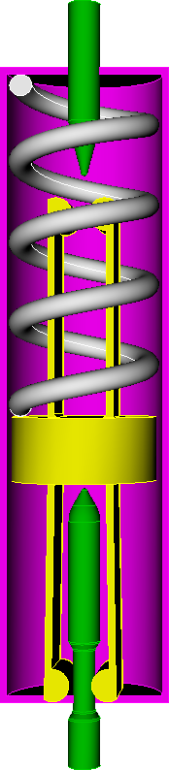
\includegraphics[scale=.2]{Acceleration_Switch.png}\end{center}
		 \caption{An example of an acceleration switch, see reference \cite{Massad2015}.}
		 \label{fig:Acceleration_Switch}
		 
		 \end{figure}	 
		
These rocket sled tests include very high velocities and accelerations, and the experiments end with their destruction upon impact. Since the test is not easily replicated, we must have the ability to consistently and correctly collect data. This means we require that the spring in the acceleration switch must function as expected to the forces exerted on it, and having a switch that is closed earlier or later than expected is undesirable~\cite{IMSM2010}. Designing a spring to behave as desired is a complicated problem that requires satisfying numerous constraints on the spring's physical properties. That the desired spring can vary depending on the application further complicates the problem. 

Spring design under these conditions amounts to a constrained optimization problem where certain properties of the spring may need to be maximized or minimized subject to bounds on some or all of the spring's other properties. Extending the scope beyond spring design for use in acceleration switches, which already cover a vast spread of specific spring designs, results in even more possibilities for design specifications. Rather than developing methods to solve these problems on an ad hoc basis, we develop to solve a wide variety of spring design problems. 

Designing an optimal spring is not a new problem. Brake et al. considered the design of an acceleration switch with enabled uncertainty~\cite{IMSM2010}. Alternatively, Sastry et al. implemented probabilistic response surface methodology to investigate the complications of uncertainty in designing a spring~\cite{Reliability}. Others have considered the reduction of the optimization problem to focus on a single parameter~\cite{Robust}. Similar tools to the ones mentioned above also exist~\cite{Paredes}.

Motivated by a workflow premise, we produce a novel tool with new capabilities. The novelties we include are the inherent flexibility in our tool's framework, tools to visualize the existence of solutions for constrained optimization problems, sensitivity analysis capabilities, and design optimization under uncertainty. We also discuss the inclusion of stress relaxation constraints in the spring design, which to our knowledge has not been considered before. We provide details regarding these items as follows. Section~\ref{sec:The_Problem} formally defines the spring design problem for helical compression springs. Section~\ref{sec:The_Approach} outlines the workflow for optimal spring design. Section~\ref{sec:Computational_Experiments} shares cases studies using our approach, and Section~\ref{sec:Summary} summarizes our work and provides suggestions for future work.

			
\section{The Problem} 
\label{sec:The_Problem}

\subsection{Helical Compression Springs}
\label{sec:Springs}

Helical compression springs, such as the one in Figure~\ref{fig:Spring}, are possibly the most recognizable type of spring and are the spring of choice for this work. 

		\begin{figure}[h]
		 \begin{center}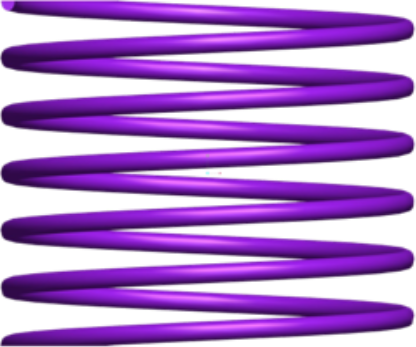
\includegraphics[scale=.2]{Spring.png}\end{center}
		 \caption{An example of a helical compression spring~\cite{Massad2015}.}
		 \label{fig:Spring}
		 
		 \end{figure}

We can uniquely define a helical compression spring by a set of design parameters, which then determine physical attributes of the spring~\cite{Massad2015}. Figures~\ref{fig:Description1}~and~\ref{fig:Description2} provide visual representations for a few of the basic parameters, and a complete list of parameters and attributes follows. 		 
		\begin{figure}[h]
			\begin{subfigure}{.5\textwidth}
				\centering
				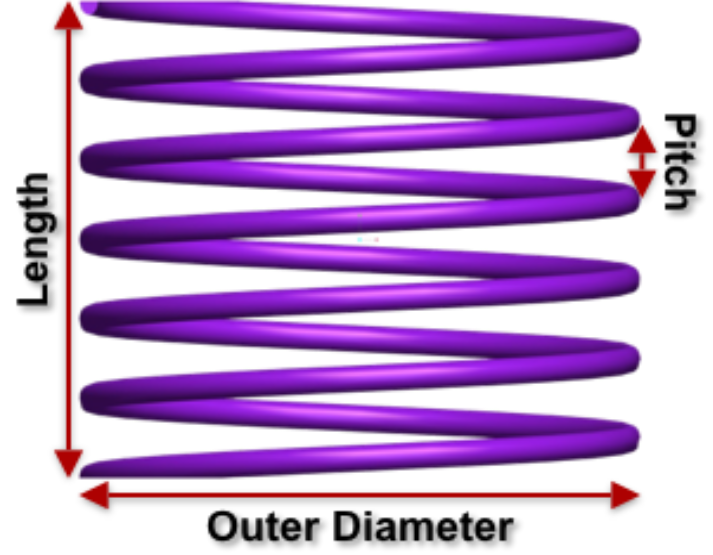
\includegraphics[scale=.17]{Spring_Description.png}
				\caption{The pitch, outer diameter, and length of a spring.}
				\label{fig:Description1}
			\end{subfigure}%
			\begin{subfigure}{.5\textwidth}
				  \centering
		 		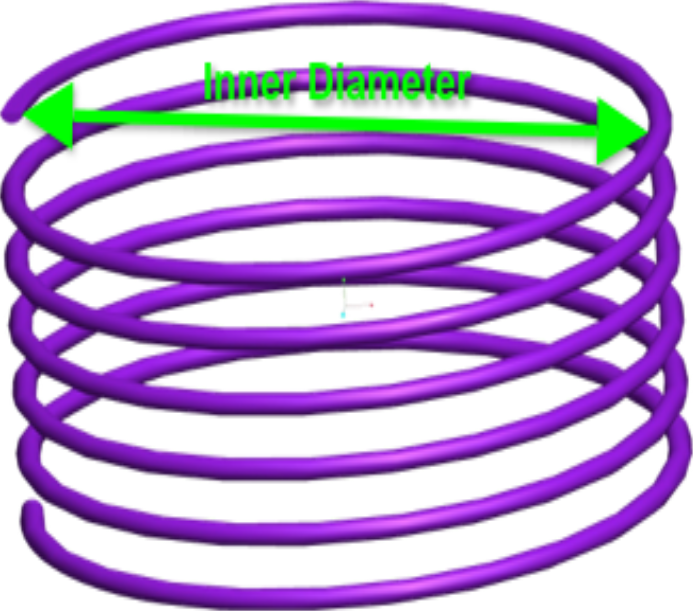
\includegraphics[scale=.15]{Spring_Description2.png}
				\caption{The inner diameter of a spring.}
				  \label{fig:Description2}
		  		
			\end{subfigure}
			 \label{fig:Descriptions}
		  \caption{A subset of basic parameters for a helical compression spring.}
		\end{figure}
		
		\center\noindent\textbf{Spring Design Parameters}
		\begin{description}[leftmargin=!,labelwidth=\widthof{\bfseries Young's Modulus (E)}]
			\item [Wire Diameter ($\boldsymbol{d}_{\text{w}}$)] This is the diameter of the circular wire used to form the spring.
		
			\item [Inner Diameter ($\boldsymbol{d}_{i}$)] This is the diameter of the circle formed by the spring's interior excluding the wire. See Figure~\ref{fig:Description2}.
			
			\item [Outer Diameter ($\boldsymbol{d}_{\text{o}}$)] This is the diameter of the circle formed by the spring including the wire, so ${d_{\text{o}} = d_{\text{i}} + 2d_{\text{w}}}$. See Figure~\ref{fig:Description1}.
			
			\item[Total Coils ($\boldsymbol{N}_{\text{t}}$)] This is the total number of 360 degree rotations formed by the spring coil. The value does not have to be an integer. 
			
			\item[Active Coils ($\boldsymbol{N}_{\text{a}}$)] This is the number of coils that contribute to the force opposing any compression force on the spring. The number of active coils depends on $N_{t}$ and the spring's end conditions. If the end condition is \textit{closed} the terminal coils of the spring are welded to their adjacent coils and $N_{a} = N_{t}-2$. If the end condition is \textit{open}, the terminal coils of the spring are free and $N_{a} = N_{t}-1$. Note this relationship creates a lower bound on the total number of coils.

			\item[Free Length ($\boldsymbol{L}_{\text{free}}$)] This is the spring's length without any force acting on it, i.e., the spring's natural length.
						
			\item[Open Length ($\boldsymbol{L}_{\text{open}}$)] This is the spring's resting length in its application. In the acceleration switch, for example, it is the length of the spring in the switch when the switch is not in use. 
						
			\item[Hard Length ($\boldsymbol{L}_{\text{hard}}$)] This is the minimum length a spring can compress to under a specified force. For the acceleration switch example, the spring cannot compression beyond a certain point under the applied forces because additional compression would reopen the circuit.
			
			\item[Solid Length ($\boldsymbol{L}_{\text{solid}}$)] This is the spring's length when its coils are completely compressed. The solid length is $L_{\text{solid}} = N_{\text{t}}d_{\text{w}}$. Also, the lengths defined must satisfy ${L_{\text{solid}} \le L_{\text{hard}} < L_{\text{open}} \le L_{\text{free}}}$.
					
			\item[Pitch ($\boldsymbol{p}$)] This is the distance between coils. For coils with \textit{closed} end conditions, ${p = \frac{L_{\text{free}}-2d_{\text{free}}}{N_{\text{a}}}}$, and for coils with \textit{open} end conditions, $p = \frac{L_{\text{free}}}{N_{\text{a}}-1}$. See Figure~\ref{fig:Description1}.			
			
			\item[Young's Modulus ($\boldsymbol{E}$)] This describes the spring's response to uniaxial stress and is one defining aspect of the spring's rigidity. Young's modulus is also know as the modulus of elasticity.
			
			\item[Poisson Ratio ($\boldsymbol{\nu}$)] This is a measurement of how much the spring deforms in any two dimensions when it is compressed in the third dimension.
			
			\item[Shear Modulus ($\boldsymbol{G}$)] This describes the spring's response to shear stress and is another defining aspect of the spring's rigidity. The shear modulus is also known as the modulus of rigidity and is $G = \frac{E}{2(1+\nu)}$. 
		
		\end{description}

		\noindent\textbf{Spring Attributes:}
			\begin{description}
				\item [Spring Rate] \begin{equation} k = \frac{G}{8N_{\text{a}}}\frac{d_{\text{w}}^{4}}{(d_{\text{i}} + d_{\text{w}})^{3}}\end{equation}
				The spring rate measures the rigidity or stiffness of the spring. 
			
			\item[Spring Index]\begin{equation}C = \frac{d_{\text{i}}}{d_{\text{w}}} + 1.\end{equation}
				The spring index measures the ratio between the spring's inner diameter and wire diameter and often is proportional to the manufacturing cost for the spring~\cite{SpringIndex}.
			
			\item[Preload Force]\begin{equation*} F_{\text{open}} = (L_{\text{free}}-L_{\text{open}})k = (L_{\text{free}}-L_{\text{open}})\frac{G}{8N_{\text{a}}}\frac{d_{\text{w}}^{4}}{(d_{\text{i}} + d_{\text{w}})^{3}} \end{equation*}
				Preload Force is the force applied to the spring while it is in the open position. For the acceleration switch example, this is the force applied on the spring when the switch is not in use.  
				
			\item[Coil Binding Gap]\begin{equation} g = \frac{L_{\text{hard}} - L_{\text{solid}}}{N_{\text{t}} - 1}\end{equation}		
				Coil binding gap is the pitch of the spring when the spring is compressed to its hard length. 
			 
			 \item[Buckling Slenderness Ratio]\begin{equation*} \lambda = \frac{L_{\text{free}}}{d_{\text{i}} + d_{\text{w}}} \end{equation*}
			 	The buckling slenderness ratio measures the spring's susceptibility to buckling under compression.
			 
			 \item[Shear Strength]\begin{equation} UTS = \frac{G(L_{\text{free}} - L_{\text{hard}})}{4 \pi N_{\text{a}}} \left[\frac{d_{\text{w}} (4d_{\text{i}}^{2} + 9.46d_{\text{i}} 
d_{\text{w}} + 3 d_{\text{w}}^{2})}{d_{\text{i}}(d_{\text{i}}+d_{\text{w}})^{3}}\right]\end{equation}
				Shear strength measures the spring's ability to withstand shear stress. 
			
			\item[Diametral Expansion]\begin{equation} d_{\text{expand}} = d_{\text{w}} + \sqrt{(d_{\text{i}} + d_{\text{w}})^{2} + \frac{p^{2} - d_{\text{w}}}{\pi^{2}}}
			\end{equation}
				The diametral expansion is the measurement of how much the outer diameter of the spring increases as the spring is compressed. Note that the discriminant of the square root is necessarily nonnegative, so diametral expansion can put additional constraints on the relationship between some parameters. 	
			% Talk about open vs closed
			
			\end{description}

This list of parameters and attributes is not exhaustive, but it does demonstrate the inherent complexities in spring design. Spring design that requires both upper and lower bounds on each of the attributes is not uncommon. As a result formulating the exact problem statement as given by the required spring design must be precise and can benefit from a standard convention. This lends itself to a mathematical formulation.

\subsection{Constrained Optimization}
\label{sec:Constrained_Optimization}

Given an input of objectives and constraints on those objectives which are both defined by a set of design variables, we can formulate the challenge of designing an optimal spring as a constrained optimization problem. The general formulation of such a problem is 
				\begin{equation*}
 					\begin{aligned}
 						& \underset{\textbf{x}}{\text{min}}
 						& & F(\textbf{x}), \\
 						& \text{subject to}
 						& & \mathbf{G}(\textbf{x}) \le \mathbf{0}.
 					\end{aligned}
				\end{equation*}
				
Here, $\mathbf{x}$ is the set of independent variables for the problem. In the context of spring design the independent variables are the spring parameters, which we also call design variables in the context of optimization. The function $F(\mathbf{x})$ is the objective function that we try to optimize. For spring design this function can consist of a single spring attribute or any weighted linear combination of attributes. Lastly, the function $\mathbf{G}(\mathbf{x})$ is the set of constraint functions restricting the optimization problem. For spring design, this set can consist of any combination of bounds on the design variables and bounds on the spring attributes.

\section{The Approach}
\label{sec:The_Approach}

Our approach follow the optimal spring design workflow illustrated in Figure~\ref{Workflow}. This is an iterative process that receives a user specified problem, reformulates and solves the problem, and then returns a result for the user to accept or decline. The remainder of this section expands upon the details of each element in this diagram.

		\begin{figure}[h!]
		 \begin{center}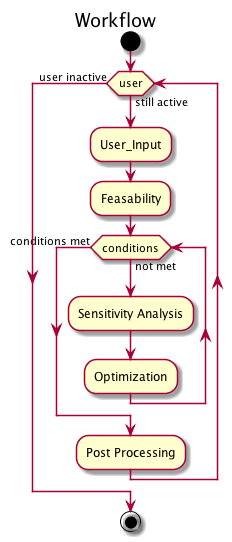
\includegraphics[scale=.4]{IMSM_Workflow.png}\end{center}
		 \caption{Illustration of the flow of our approach.}
		 \label{Workflow}
		 
		 \end{figure}

\subsection{User Input}
\label{subsec:User_Input}

The first step in our work flow is receiving spring design specifications from a user interested in building a spring for use in some industrial application.  The application will typically involve a set of attributes (eg. spring rate) to optimize and some design constraints (eg. the spring's height or diameter).  For example, consider the acceleration switch discussed during the introduction.  In this case, the user would like to achieve the smallest possible spring rate and spring index, while satisfying the physical dimensions of the acceleration switch.

\subsection{Problem Definition}
\label{sec:Problem_Definition}

Once the user has provided their input, the next step is formulating the problem.  This requires specifying an optimization objective, design variables and constraints.  To reduce the size of the permissible problem space, the user must specify the optimization function as a weighted sum of minimums and maximums.  While there are other methods for multicriteria optimization, including these in our scheme has been left to future work.  Also, we have reduced the space of design variables based on discussions with engineers experienced with spring design.

After formulating the problem, a library of predefined constraints and objectives is called to initialize the optimization software.  In some problems, however, the designer may need to constrain or optimize an attribute that is not part of the existing library.  If the user has a mathematical formulation for the desired attribute, it can be added to the constraint library for use in the problem formulation.

Our team's integration of stress relaxation provides a useful example of this process.  In some design problems, relaxation is an important objective or constraint.  To our knowledge, however, there are no spring design processes which accounting for the effects of relaxation.  Thus, our team undertook a study of stress relaxation to find a mathematical formulation (see Appendix-xx for technical details) which was added to the function library and can now be used in any problem formulation.

To allow the user maximum flexibility in their problem formulation, our software uses an object oriented design.  Object-oriented programming is an approach to software design that centers around classes which are data containers capable of performing a predefined set of tasks.  For example, our program has a \textbf{Constraint} class that includes the constraint's function, and a way to check whether the constraint is violated at a given point. For an few examples of classes see figure \ref{fig:Classes}. 

\begin{figure}[h]
			\begin{subfigure}{.5\textwidth}
				\centering
				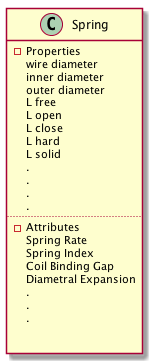
\includegraphics[scale=.5]{Spring_Class.png}
				\caption{Class for the spring}
				\label{fig:Spring_Class}
			\end{subfigure}%
			\begin{subfigure}{.5\textwidth}
				  \centering
		 		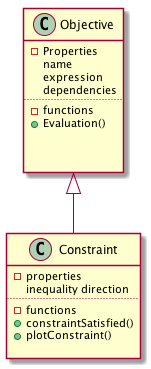
\includegraphics[scale=.5]{Objective_Constraint.png}
				\caption{Objective and Constraint Classes}
				  \label{fig:Objective_Constraint}
		  		
			\end{subfigure}
			 \label{fig:Classes}
		  \caption{A few of the classes we use.}
		\end{figure}


Using classes allow flexibility because the program's algorithm are designed to operate on the classes.  For example, the \textbf{OptimizationProblem} class generates the input for the optimizer and sensitivity analysis.  When the user inputs a new problem, the program generates an \textbf{OptimizationProblem} with a specific optimization function and set of constraints.  Thus, once the user has a problem formulation, our software can convert their problem into the objects needed for the optimizer to run.

% Check capitalization
\subsection{Feasibility}
\label{subsec:Feasibility}

Once the user has set a problem, the next step is determining the nature of the feasible region.  To assess feasibility, we use a Latin hypercube sampling method, which is designed to ensure sampling coverage over the entire domain.  This approach is used because the user defined constraints are very general in nature (for example, they can be linear or non-linear).  If a feasible point cannot be identified, the algorithm terminates and informs the user that a feasible point cannot be found.  At this point, the user can try a more exhaustive search or reformulate the problem.

Additionally, a graphical tool has been added to help the user analyze the problem's feasible region and the value of the objective function over the region.  As illustrated in the case studies, a plot with two or three state variables can be displayed highlighting the problem's overall feasible region and the contributions from each individual constraint.  This will allow the user to identify the nature of the constraints in their problem.

\subsection{Sensitivity Analysis}
\label{subsec:Sensitivity}
\hspace{5 mm} As the dimension of design variable space increases, the computational expense of the optimization procedure increases. To reduce the computational expense, it is often desirable to reduce the design variable space by removing the variables that have very little influence on the objective function. Thus, a dimension reduction strategy is required to reduce the design variable space. Dimension reduction approaches have been divided into two categories - (1)filter approach \cite{Bioinformatics}, and (2)wrapper approach \cite{Wrappers}. In the filter approach, the input variables are ranked according to a ranking criterion and the most dominant variables can be selected by assuming a threshold influence value. In the wrapper approach, a subset of variables is selected from the list of all possible subsets of the input variables that best estimate the output variable. Sensitivity analysis, a filter approach, is used in this work for dimension reduction. Two types of sensitivity analysis have been developed in the literature - local sensitivity analysis and global sensitivity analysis. The local sensitivity index of a variable measures the sensitivity of the model output when the variable is fixed at a single value whereas the global sensitivity (GSA)\cite{Global} index measures the variation of model output when the variable is varied over its range. Therefore, GSA is used as it considers the entire range instead of conditioning at a point in computing the sensitivity to the output. Note that the input variables represent the design variables and model represents the objective function.
Consider a objective function, $G$, with $n$ design variables given by $x_{1}$, $x_{2}$, ...  $x_{n}$, given by

\centerline{$Y = G(x_{1}, x_{2}, ... x_{n})$}

In GSA, two types of indices can be calculated for each variable - first order index and total effects index. The first-order index ($S_{i}^{I}$) quantifies the uncertainty contribution of an input variable, without considering its interactions with other variables, to the output variable uncertainty. Similarly, the total effects index ($S_{i}^{T}$) quantifies the uncertainty contribution of an input variable by considering its interactions with all variables, to the output uncertainty. The expressions for the two sensitivity indices are given below as 

\centerline{$S_{i}^{I} = \dfrac{V_{x_i}(E_{x_{-i}}(Y|x_{i}))}{V(Y)}$}
\centerline{$S_{i}^{T} = \dfrac{E_{x_{-i}}(V_{x_{i}}(Y|x_{-i}))}{V(Y)}$}

Given a design range (lower and upper bounds), a variable can be assumed to be uniformly distributed in the design range. For each variable, the first-order index is calculated and if it is less than an assumed threshold value, then that variable is assumed insensitive and removed from the optimization procedure. A nested double loop Monte Carlo sampling approach is adopted for computation of sensitivity indices. Note that sensitivity analysis requires a considerable computational expense and therefore may be carried out in high dimensional design optimization problems. In problems with lower number of design variables, the sensitivity analysis can be avoided and directly perform design optimization. 

\subsection{Design Optimization}
\label{subsec:Optimization}
\hspace{5 mm} A general constrained design optimization problem can be formulated as follows

\centerline{$Min \hspace{2 mm} F(\textbf{x})$}
such that

\centerline{$G(\textbf{x}) \leq 0$}
\centerline{$lb_{\textbf{x}} \leq \textbf{x} \leq ub_{\textbf{x}}$}

\noindent  Several optimization algorithms (both local and global) are available to solve the above optimization problem. DIRECT is one of the most popular global search optimization algortihm \cite{DirectUserGuide} and   \cite{DirectPaper} have been tried for this spring optimization problem.\\

The main idea of DIRECT algorithm is that  the domain is normalized to be unit hypercube and the function is evaluated at the center point $c$ of this hypercube and at points $\{c + \delta, c, c - \delta\} $ ($\delta$ is the size of the hypercube) ; then the hypercube with the smallest function value one is chosen and further divided into smaller hypercubes until the global optimum is obtained. DIRECT is a sampling optimization algorithm. It requires no knowledge of the objective function such as gradient and hessian. Since it is a global algorithm, it does not require an initial point.  Moreover, it is easy to implement in an automated software framework since it does not require segregation of linear and non-linear constraints.

\hspace{5 mm} It is also essential to account for the variability in the manufacturing process(tolerance) in the design of springs. The tolerance can also be referred to as error, uncertainty in the design variabes. The tolerance for each of the spring parameters is nominally assumed to be equal to 1\% of the value of the variable. Thus, each variable follows a uniform distribution with unknown mean and variance, dependent on the mean value. The optimization formulation after accounting for tolerances can now be written as 

\centerline{$Min \hspace{2mm} \mu_{F} (\textbf{x},d)$}

such that

\centerline{$Pr(g_{i}(\textbf{x},d) \leq 0)\geq p_{t}^{i}$}
\centerline{$Pr(\textbf{x} \geq lb_{\textbf{x}})\geq p_{lb}$}
\centerline{$Pr(\textbf{x} \leq ub_{\textbf{x}})\geq p_{ub}$}
\centerline{$lb_{d} \leq d \leq ub_{d}$}

\noindent where $\mathbf{x},d$ represent the design variables with tolerances and non-design variables with tolerances respectively. The first constraint represents the probabilistic inequality constraint and the other constraints represent the bounds for the design variables. Optimization with tolerance is a nested double loop process where optimization is carried out in the outer loop (using DIRECT)and in each iteration of optimization, reliability analysis is carried out in the inner loop using Monte Carlo sampling to check the probabilistic constraints. After obtaining the optimum values of the means of the design variables, their corresponding probability distributions can be obtained, since it is assumed that the variables follow uniform distributions with variances dependent on the mean values. 


\begin{flushleft}
\hspace{5 mm} Since the optimum design parameters are stochastic, the optimum value of the objective function, which is a function of the optimum design variables is also stochastic. The probability distribution of the optimum value objective function is obtained from the probability distributions of the design variables through uncertainty propagation analysis using Monte Carlo sampling. One random realization of each of the design parameters when passed through the objective function provides one realization of the optimum value of the objective function. Thus several realizations of design variables are obtained which result in several realizations of the optimum value of the objective function. Using the realizations, the Gaussian kernel density approach is used to construct the probability distribution.

\end{flushleft}

%\subsection{Post Processing}
%\label{subsec:Post_Processing}

\section{Computational Experiments}
\label{sec:Computational_Experiments}

\subsection{Case 1:}
\label{subsec:Case1}
%Case_56_38910

\begin{description}[leftmargin=!,labelwidth=\widthof{\bfseries State Variables:}, labelindent = 1cm]
 	\item [Objectives:] Minimize spring rate and spring index.\\

	\item[Constraints:] Inner diameter and outer diameter relation, relation on the inner, wire, and outer diameters, coil binding gap, buckling slenderness, and maximum shear stress. \\
	\item[State Variables:] $d_{i}$, $d_{w}$, and $N_{t}$ \\
\end{description}

	\subsubsection{User Input}
	
\begin{center}
	 \begin{tabular}{| c  | c |  }
	 	\hline Name & Value\\
	 	\hline G & 77 GPa \\
		\hline UTS & .7GPa \\
		\hline $g_{min}$ & .5 mm\\ 
	 	\hline $k_{max}$ & 20\\
		\hline $C_{max}$ & 10\\
		\hline $L_{free}$ & 85.5 mm\\
		\hline $L_{hard}$ & 20 mm\\
		\hline
	 \end{tabular}
\end{center}

	

	\subsubsection{Problem Definition}
	
	\centerline{$Min$ \hspace{2 mm}$0.5 \times(k/k_{max}) + 0.5 \times (C/C_{max})$}
	\begin{center}such that \end{center}
	\centerline{$d_{i} + 2 \times d_{w} \leq 60e-3$}
	\centerline{$g_{min} - \dfrac{L_{hard} - N_{t}d_{w}}{N_{t}-1} \leq 0$}
	\centerline{$\dfrac{L_{free}}{d_{i} + d_{w}} - \pi \sqrt{\frac{2(2 \nu + 1)}{\nu + 2}} \leq 0$}
	\centerline{$\frac{G(L_{free} - L_{hard})}{4 \pi (N_{t} - 2) } \left[\frac{d_{w} (4d_{i}^{2} + 9.46d_{i} 
d_{w} + 3 d_{w}^{2})}{d_{i}(d_{i}+d_{w})^{3}}\right] - UTS \leq 0$}
    \centerline{$20e-3 \leq d_{i} \leq 30e-3$}
    \centerline{$1e-3 \leq d_{w} \leq 5e-3$}
    \centerline{$9 \leq N_{t} \leq 17$}
    
\begin{flushleft}
In this case study, $\textbf{x}$ is a $3 \times 1$ vector, where $x_{1}$, $x_{2}$ and $x_{3}$ represents the inner diameter ($d_{i}$), wire diameter ($d_{w}$) and total number of coils $N_{t}$ respectively.

\end{flushleft}
    
\newpage
	
	\subsubsection{Feasibility}
	
			\begin{figure}[h!]
		 \begin{center}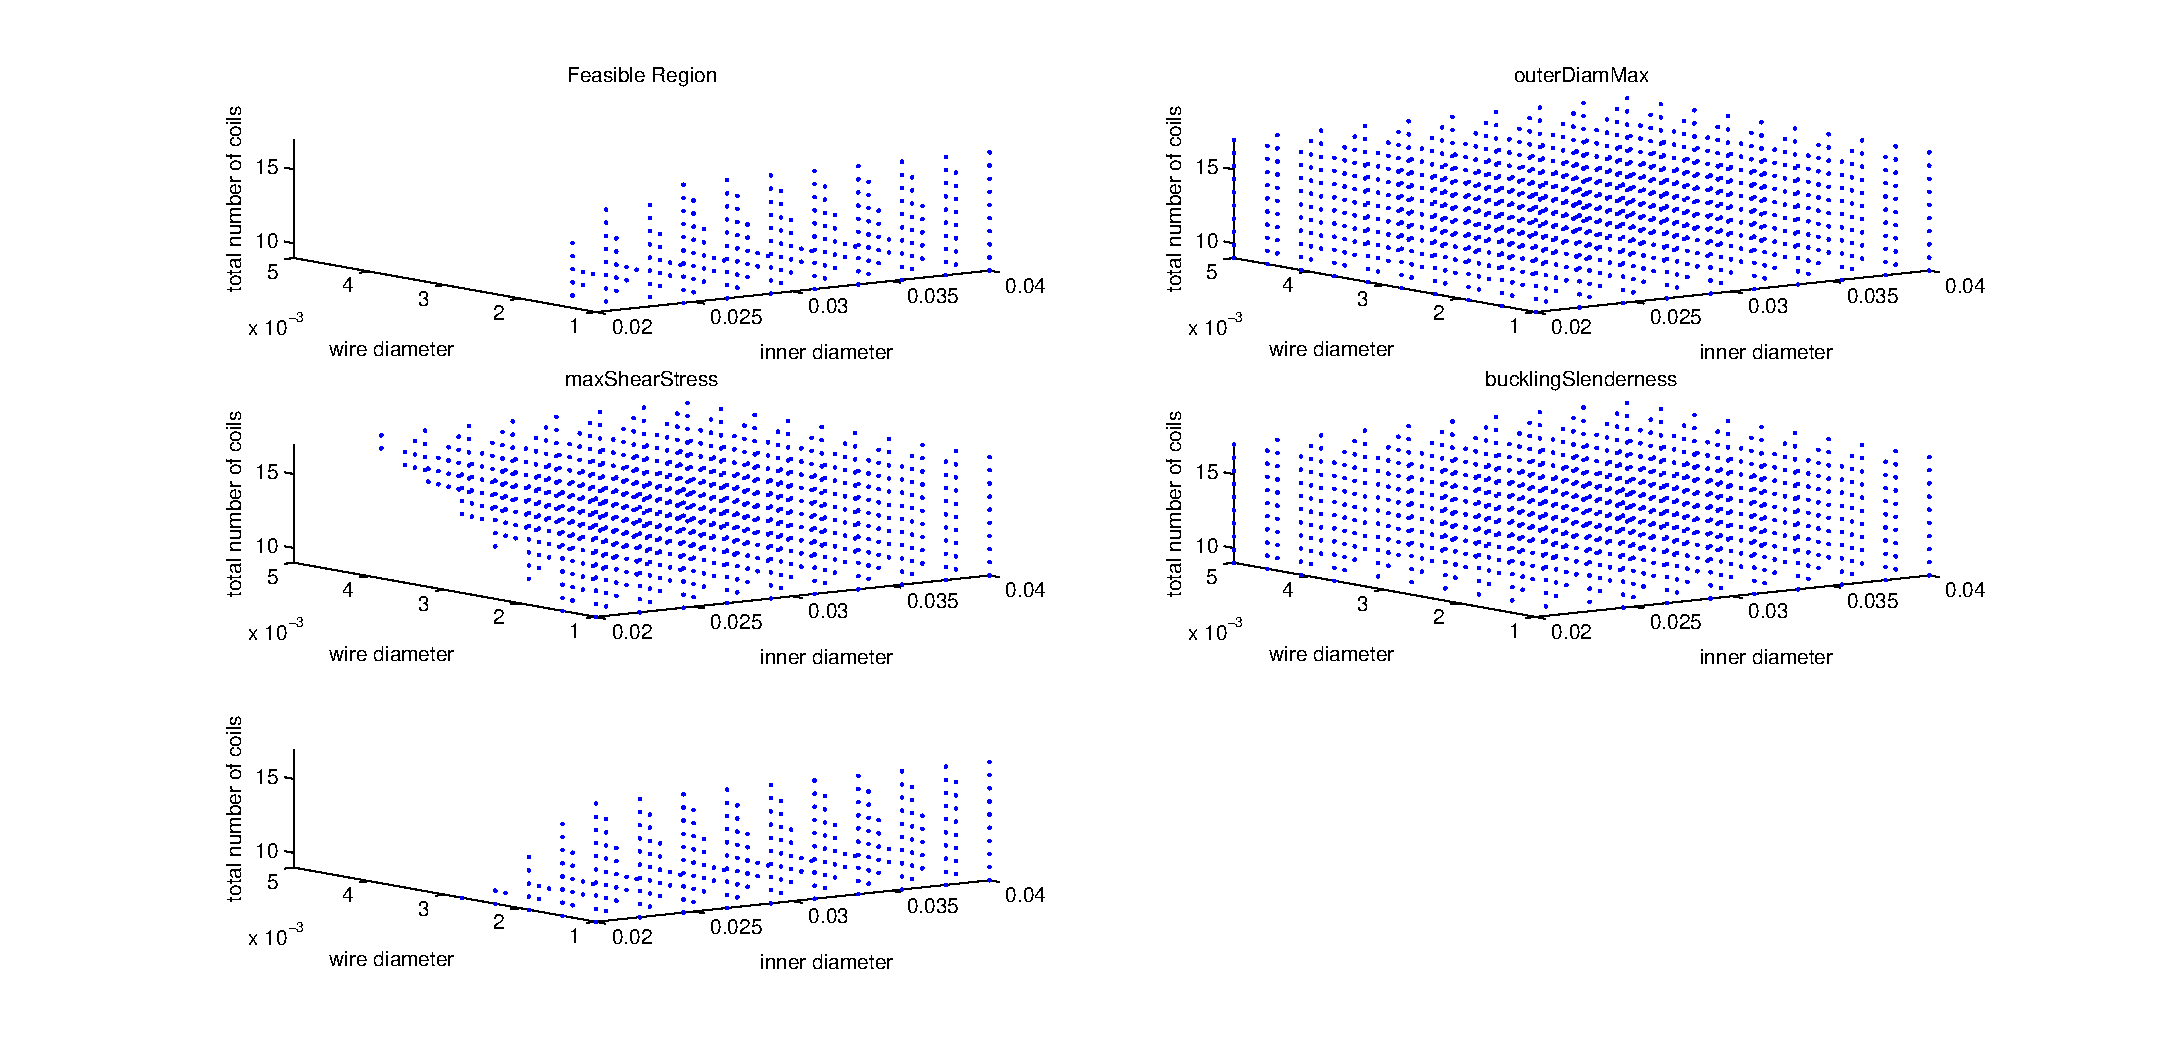
\includegraphics[scale=.35]{Case_56_38910_Feasibility.eps}\end{center}
		 \caption{Feasibility region for case 1.}
		 \label{Feasibility region for case 1.}
		 \end{figure}

	
	\subsubsection{Sensitivity}
	
\begin{center}
	 \begin{tabular}{| c  | c |  }
	 	\hline Variable & Sobol Index\\
	 	\hline $d_{i}$ & 0.16 \\
		\hline $d_{w}$ & 0.61  \\
		\hline $N_{t}$ & 0.02 \\ 
		\hline
	 \end{tabular}
\end{center}

From the sensitivity indices, it can be observed that all the design variables have significant influence on the objective function; therefore no dimension reduction is implemented for design optimization. 

	\subsubsection{Optimization}
	
	As stated in Section \ref{sec:Optimization}, DIRECT algorithm is used for optimization and the optimum design point is obtained as 
	\begin{center}
	$\mathbf{x_{opt}} =
	\left[
	\begin{array}{c}
	 	 .03 \\
	 	 .001 \\
		 17    \\ 
		
	 \end{array}
	 \right]
$	
\end{center}
    Therefore, the optimum inner diameter($d_{i}$), optimum wire diameter ($d_{w}$), and optimum number of coils ($N_{t}$) are $30 mm$, $1 mm$ and $17$ respectively.
	
	
	
	

\newpage
\subsection{Case 2:}
\label{subsec:Case2}
%Case_56_3891011

\begin{description}[leftmargin=!,labelwidth=\widthof{\bfseries State Variables:}, labelindent = 1cm]
	\item[Objectives:] Minimize spring rate and spring index.\\
	\item[Constraints:] Relation on inner, wire, and outer diameter, diametral expansion, coil binding gap, buckling slenderness, and maximum shear stress, stress relaxation. \\
	\item[State Variables:] $d_{i}$, $d_{w}$, and $N_{t}$ \\
\end{description}

	\subsubsection{User Input}
	
\begin{center}
	 \begin{tabular}{| c  | c |  }
	 	\hline Name & Value\\
	 	\hline G & 77 GPa \\
		\hline UTS & .7GPa \\
		\hline $g_{min}$ & .5 mm\\ 
	 	\hline $k_{max}$ & 20\\
		\hline $C_{max}$ & 10\\
		\hline $L_{free}$ & 85.5 mm\\
		\hline $L_{hard}$ & 20 mm\\
		\hline Norton Bailey $c$& $ 3.5 \times 10^{-6}$ \\
		\hline Norton Bailey $n$ & 1.5\\
		\hline Norton Bailey $k$ & 1 \\
		\hline Minimum Stress Relaxation & 0.85\\
		\hline Deflection $s$ & 30 mm\\
		\hline Time Stress Relaxation $t$  & $3 \times 10^{6}$\\
		\hline Stress Relaxation $G_{sr}$ & 60 GPa\\
		\hline
	 \end{tabular}
\end{center}

	\subsubsection{Problem Definition}
	
	\centerline{$Min$ \hspace{2 mm}$0.5 \times(k/k_{max}) + 0.5 \times (C/C_{max})$}
	\begin{center}such that \end{center}
	\centerline{$d_{i} + 2 \times d_{w} \leq 60e-3$}
	\centerline{$g_{min} - \dfrac{L_{hard} - N_{t}d_{w}}{N_{t}-1} \leq 0$}
	\centerline{$\dfrac{L_{free}}{d_{i} + d_{w}} - \pi \sqrt{\frac{2(2 \nu + 1)}{\nu + 2}} \leq 0$}
	\centerline{$\frac{G(L_{free} - L_{hard})}{4 \pi (N_{t} - 2) } \left[\frac{d_{w} (4d_{i}^{2} + 9.46d_{i} 
d_{w} + 3 d_{w}^{2})}{d_{i}(d_{i}+d_{w})^{3}}\right] - UTS \leq 0$}
    \centerline{$20e-3 \leq d_{i} \leq 30e-3$}
    \centerline{$1e-3 \leq d_{w} \leq 5e-3$}
    \centerline{$9 \leq N_{t} \leq 17$}
    
 \centerline{${4\over G_{sr}\theta d_w^4}\int_0^{d_w} r^2 \left( (G_{sr}\theta r)^{-n} + {c\over k} G_{sr}nt^k \right)^{-{1\over n}} \,\mathrm{d} r \ge .85$}
%\begin{center} where $\theta = {2s\over \pi N_a (d_i+d_w)^2}$ \end{center}
\centerline{where $\theta = {2s\over \pi N_a (d_i+d_w)^2}$}

\begin{flushleft}
Similar to the first case study, $\textbf{x}$ is a $3 \times 1$ vector, where $x_{1}$, $x_{2}$ and $x_{3}$ represents the inner diameter ($d_{i}$), wire diameter ($d_{w}$) and total number of coils $N_{t}$ respectively.
\end{flushleft}


\newpage
\subsubsection{Feasibility}
	
			\begin{figure}[h!]
		 \begin{center}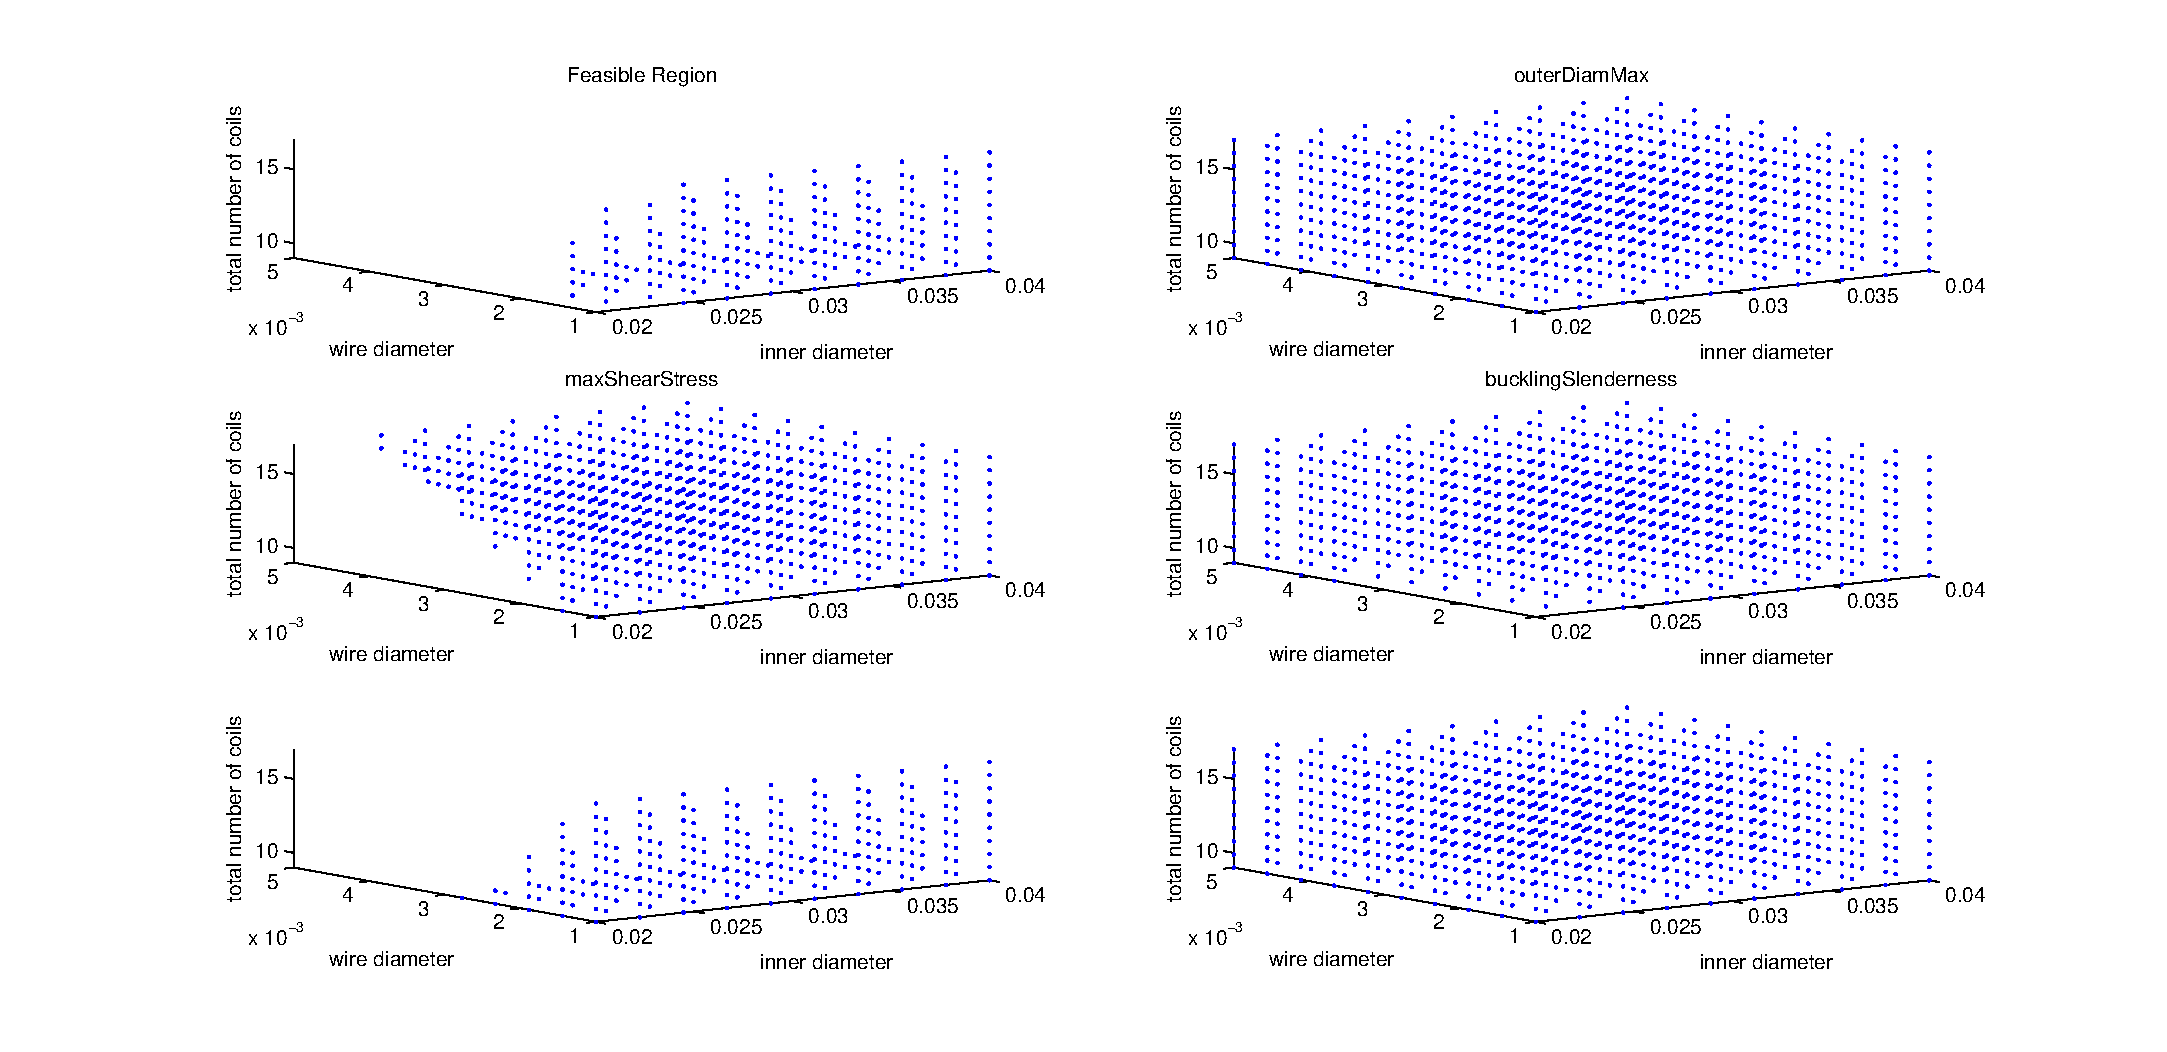
\includegraphics[scale=.35]{Case_56_3891011_Feasibility.eps}\end{center}
		 \caption{Feasibility region for case 1.}
		 \label{Feasibility region for case 1.}
		 \end{figure}
		 
\subsubsection{Sensitivity}		
 
		 \begin{center}
	 \begin{tabular}{| c  | c |  }
	 	\hline Variable & Sobol Index\\
	 	\hline $d_{i}$ & 0.19 \\
		\hline $d_{w}$ & 0.64  \\
		\hline $N_{t}$ & 0.02 \\ 
		\hline
	 \end{tabular}
\end{center}

From the sensitivity indices, it can be observed that all the design variables have significant influence on the objective function; therefore no dimension reduction is implemented for design optimization. 


\subsubsection{Optimization}
	
	As stated in Section \ref{sec:Optimization}, DIRECT algorithm is used for optimization and the optimum design point is obtained as 
	\begin{center}
	$\mathbf{x_{opt}} =
	\left[
	\begin{array}{c}
	 	 .03 \\
	 	 .001 \\
		 17    \\ 
		
	 \end{array}
	 \right]
$	
\end{center}
    Therefore, the optimum inner diameter($d_{i}$), optimum wire diameter ($d_{w}$), and optimum number of coils ($N_{t}$) are $30 mm$, $1 mm$ and $17$ respectively. Even though an additional constraint about stress relaxation is added, the optimum solution remained the same. Therefore, the assumed stress relaxation constraint does not influence the optimum solution.
    
    

\newpage
%
%\subsection{Case 3:}
%\label{subsec:Case3}
%%Case_7_348910
%	\textbf{Objectives:} Minimize force at open position.\\
%	\textbf{Constraints:} Relation on inner, wire, and outer diameter, diametral expansion, coil binding gap, buckling slenderness, and maximum shear stress. \\
%	\textbf{State Variables:} $d_{i}$, $d_{w}$, and $N_{t}$ \\
%
%\newpage
%\subsection{Case 4:}
%\label{subsec:Case4} 
%%Case_11_348
%
%	
%	\textbf{Objectives:} Maximize stress relaxation\\
%	\textbf{Constraints:} Relation on inner, wire, and outer diameter, diametral expansion, and coil binding gap. \\
%	\textbf{State Variables:} $d_{i}$, $d_{w}$, and $N_{t}$ \\
%
%
%
%		\begin{figure}[h]
%		 \begin{center}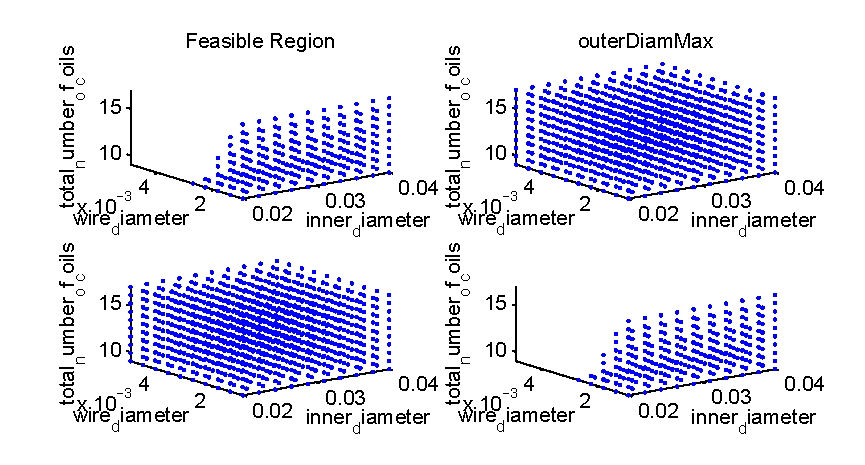
\includegraphics[scale=.75]{Case_11_348.eps}\end{center}
%		 \caption{Feasible region for case 4.}
%		 \label{Feasible Case 4}
%		 
%		 \end{figure}
% 		\textbf{Axes need to be worked on.}
%
%\newpage
%\subsection{Case 5:}
%\label{subsec:Case5}
%%Case_511_34810
%
%	\textbf{Objectives:} Minimize spring rate and maximize stress relaxation.\\
%	\textbf{Constraints:}  Relation on inner, wire, and outer diameter, diametral expansion, coil binding gap, and maximum shear stress. \\
%		\textbf{State Variables:} $d_{i}$, $d_{w}$, and $N_{t}$ \\
%		
%				\begin{figure}[h!]
%		 \begin{center}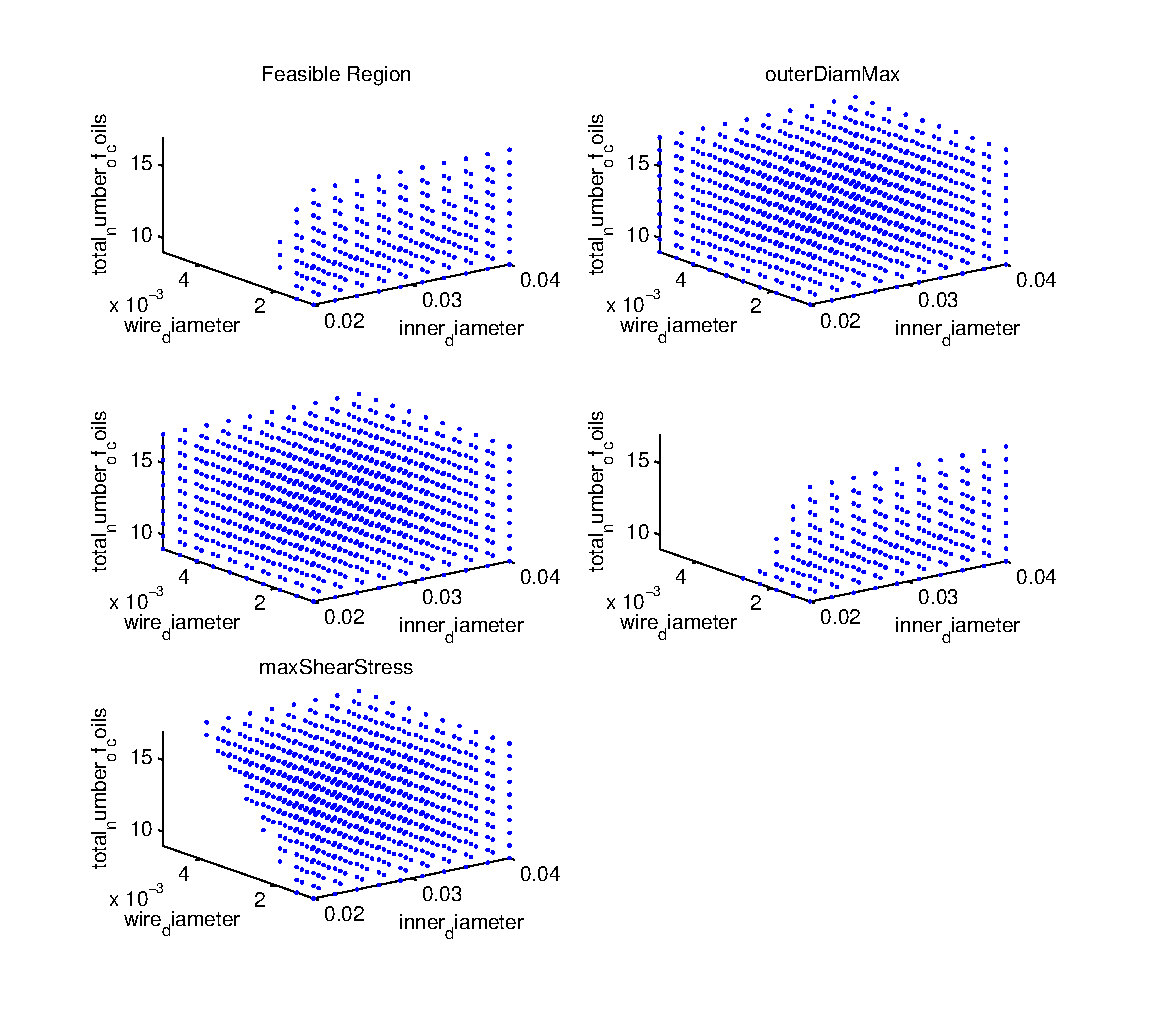
\includegraphics[scale=.50]{Case_511_34810.eps}\end{center}
%		 \caption{Feasible region for case 5}
%		 \label{Feasible Case 5}
%		 
%		 \end{figure}
%		 \textbf{Axes need to be worked on.}
%
%\newpage
%\subsection{Case 6:}
%\label{subsec:Case6}
%%Case_58_3468910
%\textbf{Saideep added a 7a, need to deal with it.}\\
%	\textbf{Objectives:} Minimize spring rate and coil binding gap.\\
%	\textbf{Constraints:} Relation on inner, wire, and outer diameter, diametral expansion, coil binding gap, buckling slenderness, and maximum shear stress. \\
%		\textbf{State Variables:}$d_{i}$, $d_{w}$, $L_{hard}$, and $N_{t}$ \\
%
%\newpage

\section{Summary and Future Work}
\label{sec:Summary}
We developed an intelligent tool for the design of helical compression springs. The key highlights of this tool are: One, it allows for flexible optimization, which enables design of springs with interchanging objective functions and constraints. Two, it can incorporate stress relaxation in the design process, which to our knowledge has never been done. Three, it provides a feasibility design space given the constraints. Four, it can provide the global sensitivity indices of the design variables to the objective function. 

Some limitations of the approach outlined are as follows. The choice of optimization and sensitivity analysis are fixed, however, they are modularized to allow a different optimization routine and sensitivity analysis to be incorporated. Given the amount of flexibility that is enabled, a user will have to be able to decide if a infeasible solution is due to user error. 

More analysis of the stress relaxation and creep could result in better performance when using those conditions. Analysis on models of stress relaxation and their performance in our model would be beneficial for both our design, and could further understanding of stress relaxation and creep.

In this work, the DIRECT algorithm for global optimization is used for the design of springs. Also, computational experiments have been carried to perform design optimization considering tolerances in design variables but not incorporated in the design tool; this is an future work of importance. Other future work is to considering faster single-loop techniques, faster analytical and sampling techniques such as First Order Reliability Methods (FORM), and Importance sampling need to be considered

% The key highlights of this tool are (1) Allows for flexible optimization, which enables design of springs with interchanging objective functions and constraints, (2)Can incorporate stress relaxation in the design process, (3) Provides a feasibility design space given the constraints, (4)Provide the global sensitivity indices of the design variables to the objective function. 
% The ability to interchange constraints and objective functions with any number of design variables allows the user the utmost flexibility. With the addition of feasibility and sensitivity analysis it is possible for any configuration of objective function, constraints, and design variables to be analyzed for refinement. The quantification of stress relaxation and creep allow the user a chance to incorporate these properties into any configuration, especially those that have never been tested. The sensitivity indices serves two purposes - help the designer understand which variables have the most influence on the objective function and also help in dimension reduction in the design space for a faster optimization.

%Provide some highlights of object-oriented programming for Spring model design
%
%A couple of sentences of stress relaxation



%In this work, the nested double-loop approach is used for global sensitivity analysis. As the dimension of design variables increases, the nested double-loop approach becomes computationally very intensive. Therefore, more faster single-loop techniques should be considered. Also, reliability analysis within the optimization procedure is carried out using Monte Carlo sampling. As the complexity of the problem increases, in terms of the number of design variables and the number of constraints, Monte Carlo sampling becomes very intensive. Therefore, faster analytical and sampling techniques such as First Order Reliability Methods (FORM), Importance sampling need to be considered.



\section{Appendix}
\label{sec:stress}
A rocket mounted spring is expected to deliver normal mechanical output under extreme temperatures. The analysis of creep behavior helps us design a spring to meet the requirements under rough conditions.

Creep is the strain increase under constant stress, usually activated by high temperatures. Three mechanisms have been proposed to account for the phenomenon: dislocation slip and climb, grain boundary sliding and diffusional flow. We focus on the creep caused by the dislocation mechanism. The material's creep tendency is determined by a creep test. During a test, the spring is kept at $0.3-0.5T_m$ ($T_m$ is the melting temperature of the material) and loaded by a constant tensile force.

Conventionally, creep can be divded into $3$ stages. In the first stage (primary/ reduced/trasient) ,the creep strain rate decreases to a certain value(minimum creep rate). The second stage(secondary/steady/stationary creep) is characterized by a nearly constant creep rate(minimum creep rate). In the third stage(tertiary creep), the creep strain rates increases rapidly and leads to rupture. The first stage is usually reversible with time after unloading, while the second/third ones are not. Since the primary creep occurs in a short duration and the tertiary one leads quickly to rupture, the secondary creep is under most serious consideration in many engineering designs.

Another common test to determine the material's susceptibility to high temperature is called stress relaxation. During the test the load is continuously decreased in such a way that the initial strain remains constant. The mechanism is more or less the same as that of creep.

\subsection{Creep rate law of material}
\label{sec:Creep}
The starting point is the assumption that the creep rate may be described as a product of three separate functions of stress, temperature and time
\[
\epsilon_{cr}(\sigma,T,t)=f_\sigma (\sigma) f_T(T) f_t(t)
\]
The widely used functions of stress $f_\sigma(\sigma)$ are (\cite{Creep}):

\begin{tabular}{ll}
$a\sigma^n$ & Norton, 1929, Bailey, 1929 \\
$b\left( \exp{\sigma\over \sigma_0} -1 \right)$ & Soderberg, 1936 \\
$a\mathop{sinh}{\sigma\over \sigma_0}$ & Prandtl, 1928, Nadai, 1938, McVetty, 1943\\
$a_1\sigma^{n_1} + a_2 \sigma^{n_2}$ & Johnson et al., 1963 \\
$a\mathop{sinh} \left( {\sigma\over \sigma_0}\right)^n$ & Garofalo, 1965
\end{tabular}

where $a,b,a_1,a_2,\sigma_0,n_1,n_2$ are material constant. The dependence on the temperature $f_T(T)$ is usually expressed by the Arrhenius law
\[
f_T(T) = \exp \left( {-Q\over RT}\right)
\]
where $Q$ and $R$ denote the activation energy and the Boltzmann's constant.

The time dependence part $f_t(t)$ is assumed to be (\cite{Ch2000}):

\begin{tabular}{ll}
$t$ & secondary creep \\
$bt^m$ & Bailey \\
$(1+bt^{1/3})\exp{kt}$ & Andrade\\
$\sum_j a_j t^{m_j}$ & Graham and Walles
\end{tabular}

For simplicity, we are going to only use the Norton-Bailey law and ignore any dependence on the temperature since the temperature is constant.
\section{Stress relaxation of helical spring}
The following section is based on the paper(\cite{Relaxation1}). Due to conservation of the total shear strain, the sum of the creep strain $\epsilon_{cr}$'s rate of change and that of elastic shear strain $\epsilon_{el}$ is zero:
\[
\dot{\epsilon}_{cr} + \dot{\epsilon}_{el} = 0
\]
Dot is meant as differentiation in time. The elastic shear strain is related to the shear stress by shear modulus $G$: $\epsilon_{el} = \sigma/G$ and taking the derivative with time on both sides, we arrive at
\[
\dot{\epsilon}_{el} = \dot{\sigma}/G
\]
According to Norton-Bailey law(also known as time hardening law),
\begin{equation} \label{eq:N-B}
\dot{\epsilon}_{cr}(t)=c\sigma^{n+1} t^{k-1}
\end{equation}
where $c$ is the shear strain rate, $n,k$ are temperature dependent material constants.

Substituting the above two equations to the conservation law,
\begin{equation} \label{eq:diff}
\dot{\sigma}(t)/G+c\sigma(t)^{n+1} t^{k-1}=0
\end{equation}
The initial condition is
\[
\sigma (0) = G\theta r
\]
where $\theta$ is the initial twist angle per unit length, $r$ the radius of wire.

\[
\sigma = \left( (G\theta r)^{-n} + {c\over k} Gnt^k \right)^{-{1\over n}}
\]

The torque can be written as
\begin{align*}
&M(t) = 2\pi \int_0^{d_w} r^2 \sigma(r,t)\,\mathrm{d} r\\
&M(0)={1\over 2} G\pi\theta d_w^4
\end{align*}
where $d_w$ is the wire diameter.

Since the spring load is linearly related the torque $P_z(t)\propto M(t)$, given the constant deflection $s$,
\[
{P_z(t)\over P_z(0)} = {M(t)\over M(0)} = {4\over G\theta d_w^4}\int_0^{d_w} r^2 \left( (G\theta r)^{-n} + {c\over k} Gnt^k \right)^{-{1\over n}} \,\mathrm{d} r
\]
where
\[
\theta = {2s\over \pi N_a ((d_i+d_o)/2)^2}
\]
The integral has no endpoint singularity and can be integrated to high order precision using the Gauss quadrature formula. The closer this quantity is to $1$, the better the spring quality is. We notice that a seemingly simpler form has been presented in the paper.
\[
{}_{2}F_1 \left( {4\over n},{1\over n};{4+n\over n};{c\theta^n G^{n+1} n t^k\over k} {d_w^n\over 2^n}\right)
\]
which we find to yield unrealistic values due to divergence issues.

\subsection{Stress relaxation of helical spring}
\label{sec:Relaxation}

Due to conservation of the total shear strain, the sum of the creep strain $\epsilon^{cr}$'s rate of change and that of elastic shear strain $\epsilon_{el}$ is zero:
\[
\dot{\epsilon}_{cr} + \dot{\epsilon}_{el} = 0
\]
The elastic shear strain is related to the shear stress by shear modulus $G$:
\[
\epsilon_{el} = \sigma/G
\]
and therefore
\[
\dot{\epsilon}_{el} = \dot{\sigma}/G
\]
According to Norton-Bailey law(also known as time hardening law),
\begin{equation} \label{eq:N-B}
\dot{\epsilon}_{cr}(t)=c\sigma^{n+1} t^{k-1}
\end{equation}
where $c$ is the shear strain rate, $n,k$ are temperature dependent material constants.

Substituting the above two equations to the conservation law,
\begin{equation} \label{eq:diff}
\dot{\sigma}(t)/G+c\sigma(t)^{n+1} t^{k-1}=0
\end{equation}
The initial condition is
\[
\sigma (0) = G\theta r
\]
where $\theta$ is the initial twist angle per unit length, $r$ the radius of wire.

\[
\sigma = \left( (G\theta r)^{-n} + {c\over k} Gnt^k \right)^{-{1\over n}}
\]

The torque can be written as
\[
M(t) = 2\pi \int_0^{d_w} r^2 \sigma(r,t)\,\mathrm{d} r ={}_{2}F_1 \left( {4\over n},{1\over n};{4+n\over n};{c\theta^n G^{n+1} n t^k\over k} {d_w^n\over 2^n}\right) M(0)
\]
where $d_w$ is the wire diameter.

Since the spring load is linearly related the torque $P_z(t)\propto M(t)$, given the constant deflection $s$,
\[
{P_z(t)\over P_z(0)} = {}_{2}F_1 \left( {4\over n},{1\over n};{4+n\over n};{c\theta^n G^{n+1} n t^k\over k} {d_w^n\over 2^n}\right)
\]
where
\[
\theta = {2s\over \pi N_a ((d_i+d_o)/2)^2}
\]
The closer this quantity is to $1$, the better the spring quality is.

\subsection{Creep of helical spring}
This section is based on the paper(\cite{Relaxation3}). The starting point is still the Norton-Bailey law (\ref{eq:N-B}). There is naturally another way to write the shear strain rate:
\[
\dot{\epsilon}_{cr} = \dot{\theta} r = {8\dot{s} r\over \pi N_a (d_i+d_o)^2}
\]
We obtain $\sigma$ from substiting the above equation into Norton-Bailey law. Given the constant spring force $P_z^0$,
\[
P_z^0{d_i+d_o\over 4}=M(0)=2\pi\int_0^{d_w} r^2 \sigma(r,t)\,\mathrm{d} r
={\pi\over 4}{n+1\over 4+3n}\left( {8d_w^{4+3n}\dot{s} \over t^{k-1} (d_i+d_o)^2 \pi N_a c (d_i+d_o)^2} \right)^{{1\over n+1}}
\]
It can be deduced that the spring length $s$ follows
\[
s(t) = s(0) + \left( {(d_i+d_o)P_z^0\over \pi}{4+3n\over n+1} \right)^{n+1} {\pi (d_i+d_o)^2 N_a c\over 8kd_w^{4+3n}} t^k
\]
where $s(0)$ is the initial spring length. The less the difference of the spring length $s(t)-s(0)$, the better the spring quality is.
 
 \cite{Ch2000} \cite{Relaxation1} \cite{Relaxation2} \cite{Relaxation3} \cite{Creep} 
\subsection{Analysis of stress relaxation and creep models}
\label{sec:stressanalysis}




\vfill\pagebreak


	
	\bibliographystyle{ieetr}

\bibliography{MyBib}



\end{document}

